\documentclass[10pt,conference,compsocconf]{IEEEtran}

\usepackage{hyperref}
\usepackage{graphicx}	% For figure environment
\usepackage{placeins}
\usepackage{float}


\begin{document}
\title{Machine Learning Project II}

\author{
  Andres Montero, Elias Poroma, Jonas J\"aggi\\
  \textit{School of Computer and Communication Sciences, EPFL, Switzerland}
}

\maketitle

\begin{abstract}
This report is the description of the different machine learning
models and approaches executed to obtain an estimation of the 
likelihood that a tweet is either positive-1 or negative-0. 
It summarizes the different text preprocessing steps and cleaning 
methods applied to obtain the highest accuracy. For this purpose, real
world data of 2,500,000 tweets is used, which is are already labeled, and also GloVe embeddings representation. Based on this and analyzing the different
results obtained, we observe that the best accuracy is obtained using a
convolutional neural network architecture which predicts N-grams for groups of words.

\end{abstract}

\section{Introduction}

Nowadays when artificial intelligence is one of the most important topics of research and applications development, it is required that machines are able to process data, specially text, and thankfully there is a great amount of this type of data that can be used to train different machine learning models. This particular field of study in artificial intelligence is called Natural Language Processing (NLP), which consists of creating a system that is able to process and understand written text in order to perform specific tasks. This project focuses on implementing a Sentiment Analysis of text extracted from the social media platform "Twitter", which brings a new challenge because of the fact that the group of people that uses this platform is completely heterogeneous and therefore can express their feelings in a variety of ways, with different abbreviations of words, emojis, hashtags, etc.
The data-set used was provided by Kaggle, and consists of a training data-set of 2,5 millions tweets labeled as either 0 for a tweet that used to contain a negative smiley or 1 for a tweet that used to contain a positive one. For the initial training of our algorithms, we use only 200000 tweets because of time it takes for the models to train, however with the insights obtained from this first training step, we then adjust our models and our cleaning functions so that we can then train the models with the full 2,5 million tweets. 
The report gives a summary of the different pre-processing steps used to clean the data, the different options for the word representation used and the different machine learning models. 
At the end the model that gave us the best accuracy and the highest score for both our validation data-set and the score in crowdAI\cite{crowdai_01} is a Convolutional Neural Network with N-grams to group words.

\section{Data representation}
In order to obtain a good text classifier, it is important to find the best feature representation of the input text. In this section we will describe the algorithms to convert the tweets into a numerical representation, in this sense the first step is to build a vocabulary that represents the words but in a numeric form.
The numeric representation methods that were used are:
\subsection{Word Embedding}
 An embedding\cite{embeddings_01} is a set of language modeling and feature learning techniques in NLP, where words or phrases form the vocabulary are mapped to vectors of real numbers. Word and phrase embeddings are used to boost the performance in NLP tasks such as syntactic parsing and sentiment analysis.
With this in mind we are using two different representation of embeddings:
\begin{itemize}

\item Own Embeddings

We are training our own embeddings by using matrix factorization to obtain the embedding matrix for our words based on the co-occurrence matrix of these words in the training tweets.

\item Using pretrained embeddings 

Another approach that we used is to use a set of embedding matrix already pretrained, in this case we used an embedding matrix which was created by the Standford University\cite{embeddings_02}. This embeddings are based on 2,6 Billion tweets.
For our purpose however we filter out only the embeddings that occurred at least 5 times in our training data set so that we can reduce its size and speed up the process of training the models.
\end{itemize}
\subsection{N-gram}
N-gram is a representation generally used in language models. A N-gram is a contiguous sequence of n items from a given sample of text or speech. In this approach the different N-gram sizes tested were n = 2,3 and 5.

\section{Text pre-processing}

In this section we will describe the different approaches used to clean the data and evaluate if this steps caused an increase or not in the accuracy of the different models trained.
In order to obtain a good model we need to first understand our training data-set, because of Twitter's nature of quick and short messages, they usually contain misspelled words, emojis, hashtags and other special characters. So the following steps where applied differently according to each model and numeric representation of the tweets in order to obtain the best accuracy.
With this information, the most important insights of the different pre-processing steps are:
\begin{itemize}

\item Remove duplicates: In the tweets we found that some tweets were duplicated, these lines of text would not help our model as it will have the exact same information, therefore we first remove the tweets that are duplicated.

\item Interpret emojis: This function is used to interpret emojis found on the text of a tweet and replace it with a word, for example replace  \texttt{<3\,},\texttt{<heart>\,}.

\item Full stop and commas: In most cases, full stops and commas do not express sentiment, so they are removed.

\item Handle numbers: In this function we tried two different approaches, the first was to remove all the numbers of the data-set. The second was to replace each number by the \texttt{<number> \,}word, which exists in the embedding and will reduce the size of the vocabulary significantly.

\item Handle special symbols : In the tweets is really common to use special simbol or special characters, so one approach was to remove all these symbols with exception of exclamation !, plus + and minus -.

\item Replacing more letters: In the tweets there also exist cases where a word is misspelled with repeated characters of the word itself, for example : haaaappy instead of happy. However we noticed that even if the word is misspelled, it has a different sentiment over the correctly spelled word, in a tweet if a user tweets haaaappy instead of just happy, the first case implies a more positive sentiment. 

\item Expand contractions: Contractions are used frequently in tweets because of the informality of shortness of the message itself, in that sense one approach is to expand this contractions to observe if this will increase the accuracy of our model, for example: "don't" is transformed to "do not".

\item Remove stop words: This method consists in removing the most common words in a language, in the project we used the nltk library~\cite{nltk01} as a reference of words to remove from the tweets, for example: "I want to go to the movies" converted into "want go movies". 

\item Correct Spelling: Tweets have a lot of abbreviations and misspelling. It may occur that a word that expresses the sentiment of the sentence is misspelled; to try to solve this issue we will correct the data-set with the use of TextBlob~\cite{Textblob01} library. 

\item Lemmatization: Lemmatization consists in converting a word into the root word. It makes use of the vocabulary and does a morphological analysis to obtain the root word. For this we used the library NLTK tokenizer and lemmatizer.

\item One Space: This method consists in removing extra spaces between words, if not the model may consider two spaces as a different word.

\item Test Data-set: All the functions presented earlier are applied to both the training and the test data-set, however because the structure of the Test data-set is different, where the number of rows are followed by a comma, we first delete this information, and after the pre-processing steps we add again the index and the comma.

\end{itemize}

\section{Baseline - Logistic regression}
As a first approach, and in order to have a baseline for comparing other models, we use logistic regression. The loss to be minimized is
\[\sum_{n=1}^{N}ln[1+exp(x^T_nw)]-y_nx_n^Tw)\]
Where we use the mean over all word vectors of one tweet to represent the features x. y $\in$ (0, 1) is the label for each tweet. y=0 means that the tweet originally had a sad smiley, and y=1 means a happy smiley. W is the weight vector, initialized as random values $w_i \in$ [0, 1]. The idea behind this approach is that some indices of the word vector represent certain feelings, and the average over all words of a tweets therefore represents some "general mood". The tuned hyper-parameters for this model are step-size $\gamma$ = 0.0001 and $\gamma$ = 0.01 for regularization. Training for the models in \ref{tab:models} is performed using stochastic gradient descent with batches of size 1000 for 60 epochs (which is equal to ~5 epochs on the whole data-set).

\begin{table}[H]
  \caption{Logarithmic regression - Accuracy in Percent for training on 190'000 tweets , while using 10'000 tweets for validation}
  \label{tab:models}
\begin{tabular}{|l|l|l|l|}
\hline
\textbf{GloVe Dimensions}                                                              & \textbf{Our GloVe} & \textbf{Pretrained GloVe}     \\ \hline
\begin{tabular}[c]{@{}l@{}}25\end{tabular}               &    59.4        & \begin{tabular}[c]{@{}l@{}}65.9\end{tabular} \\ \hline
\begin{tabular}[c]{@{}l@{}}50\end{tabular}               &    60.2        & \begin{tabular}[c]{@{}l@{}}66.3\end{tabular} \\ \hline
\begin{tabular}[c]{@{}l@{}}100\end{tabular}               &    60.6        & \begin{tabular}[c]{@{}l@{}}68.3\end{tabular} \\ \hline
\begin{tabular}[c]{@{}l@{}}200\end{tabular}               &    62.1        & \begin{tabular}[c]{@{}l@{}}70.3\end{tabular} \\ \hline
\end{tabular}
\end{table}
 
Using the pretrained word vectors consistently yields much better accuracy on the same model. This is probably due to the fact that they have been trained on a much bigger data-set than ours. Increasing the dimensions of the embeddings is beneficial, especially for the pretrained embeddings, by far. When training on the whole data-set for 5 epochs, we achieve an accuracy of 77.2\%.

\section{Convolutional Neural Nets}

Convolutional neural nets (CNN) are often used in Computer Vision. A convolutional network layer is like a sliding window, which computes the convolution of a subset of pixels with a kernel containing trainable weights. The same principle can be applied to a sequence of words: In this case, the kernel has size $[m] * [embedding\_dimensions] $, where m is the number of words we want combine. The output of the layer is the convolution of the embedding vectors of these n words, as a scalar. Advantages of CNNs in NLP are \textit{Location invariance} and \textit{Compositionality} \cite{britz_2016}. The result is invariant to the position of a group of word in the whole collection off words (or in a tweet in our case). Compositionality means that instead of interpreting each word separately, we learn the interpretation of a group of words instead of the meaning of each word on its own. 

 Input data contains only the index of the words of a tweet in the embedding matrix. It is preferable to have constant input size, because this allows us to feed multiple tweets at once into the training procedure in the form of mini-batches. This way, we can profit from the speed advantage of computing in parallel. Once the tweet with the highest word count is determined, we pad the other tweets with zero embeddings in order to reach the same size. The net contains an embedding layer, which then computes the embeddings for each tweet. Technically it is possible to include this embedding layer in the back-propagation, and thereby make the embeddings trainable as well. We block the parameters of the embedding layer, as training them doesn't significantly improve our results.
 
 \subsection{Network architecture}
 
 \begin{figure}[H]
  \centering
  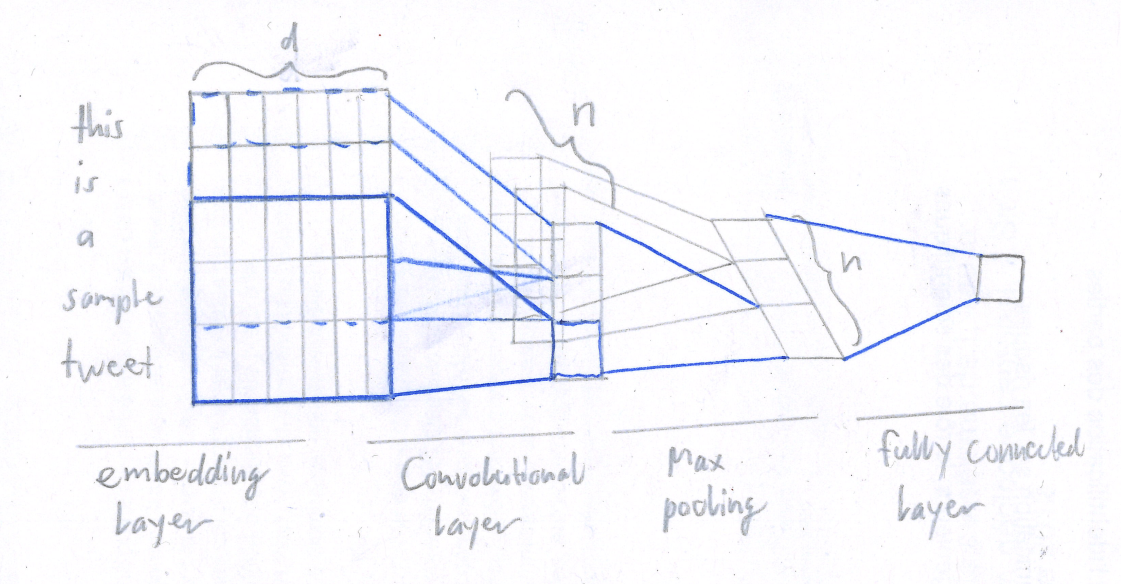
\includegraphics[width=\columnwidth]{network_architecture.png}
  \caption{Architecture of the simple convolutional net approach.}
  \vspace{-3mm}
  \label{fig:network_architecture}
\end{figure}

\begin{itemize}
    \item 
    \textbf{SimpleConvNet} (Figure \ref{fig:network_architecture})
    A convolutional layer is applied to each group of 3 words. The values of these convolutions form a vector representing the 3-Grams of the tweet. This is done multiple times with different weights in the convolutional kernel, forming an array of n tweet vectors. We refer to these n vectors as channels, because of the similarity to convolutional channels in computer vision. The convolutional layer is followed by a ReLu activation function. The maxima of these rectified values for each channel are then forwarded together through a fully connected linear layer, reducing the representation of the tweet to a scalar. The label is then the rounded value of the sigmoid function on this scalar.
    \item
    \textbf{ClassificationNet}
    SimpleConvNet is basically tackling the problem as a regression on a scale from 0 (sad) to happy (1). ClassificationNet uses the same layers as SimpleConvNet, but instead of having one scalar output, it has two: One value for sadness, and one for happiness, each representing the probability by which the tweet belongs to one category or the other. It treats the task as a classification problem. To determine the label, we use the softmax function:
    \[\sigma(z)_j=\frac{e^{z_j}}{\sum_{k=1}^{K}e^{z_k}}\]
    The softmax function transforms a vector of real values $z = [z_{sad}, z_{happy}]$ into a vector $\sigma(z) = [\sigma_{sad}, \sigma_{happy}]$ containing only zeros and ones, in a way that the sum over all elements is 1, so only the element with the highest probability will have the value 1. The label is then the index of the element with value 1.
    \item
    \textbf{N-grams} This approach extends SimpleConvNet by adding two convolution layers with filters of size m=2 and m=5. This approach (not with these specific filter sizes) is proposed by \cite{bentrevett}. It learns the 2-, 3- and 5-grams of the word combinations in the tweets. The three convolution layers operate in parallel, and instead of n tweet vectors we now have 3*n vectors. Again max pooling and a fully connected layer are used to regress to a single scalar.
    
\end{itemize}

\begin{table}[H]
  \caption{Comparison between the performance of the net architectures. Nets are trained on 190'000 tweets for 5 epochs, using batches of 1024 tweets. Validation accuracy is estimated using 10'000 tweets of the data-set.}
\begin{tabular}{|l|l|l|l|}
\hline
\textbf{\begin{tabular}[c]{@{}l@{}}Net\\ {[}channels{]}\end{tabular}} & \textbf{\begin{tabular}[c]{@{}l@{}}Validation\\ Accuracy (\%)\end{tabular}} & \textbf{\begin{tabular}[c]{@{}l@{}}CrowdAI\\ Score (\%)\end{tabular}} & \textbf{\begin{tabular}[c]{@{}l@{}}Time per\\ Minibatch (s)\end{tabular}} \\ \hline
N-grams {[}64{]} & 84.2 & 83.4 & 130 \\ \hline
\begin{tabular}[c]{@{}l@{}}ClassificationNet\\ {[}64{]}\end{tabular} & 83.4 & 83.0 & 60 \\ \hline
\begin{tabular}[c]{@{}l@{}}SimpleConvNet\\ {[}16{]}\end{tabular} & 82.8 & 82.4 & 40 \\ \hline
\begin{tabular}[c]{@{}l@{}}SimpleConvNet\\ {[}64{]}\end{tabular} & 83.4 & 82.8 & 60 \\ \hline
\begin{tabular}[c]{@{}l@{}}SimpleConvNet\\ {[}256{]}\end{tabular} & 83.8 & 83.1 & 120 \\ \hline
\begin{tabular}[c]{@{}l@{}}SimpleConvNet\\ {[}1024{]}\end{tabular} & 84.7 & 83.4 & 530 \\ \hline
\end{tabular}
\end{table}

The N-grams architecture seems to perform best. There is no significant difference in accuracy between classification and regression in the case of only two classes. Furthermore, increasing the channel count is beneficial up to a certain point. However, the number of network parameters is directly proportional to the number of channels. Therefore, computational time increases accordingly. For our final submission, we train the N-grams net on the whole dataset (2'500'000 tweets) for 5 epochs, again using batches of 1024 tweets.

 \subsection{Measures against over-fitting}
 We use L2 regularization on the weights of our network layers, but we can still see artifacts of over-fitting: at some point, while the loss is still getting reduced, the accuracy of the predictions on the validation set can decrease again. This is illustrated by the continuous blue line in Figure~\ref{fig:Validation accuracy vs Loss}.
 
 A technique that can be applied to avoid over-fitting is dropout \cite{budhiraja_2016}. The name stands for a procedure during which each time we forward through our net layers during training, a set of neurons (chosen at random, with a fixed probability p) is deactivated, which means that they will not contribute to the output of this round. When forwarding the features through the net in order to predict outputs, all neurons are active, but their output will be scaled by p in order to compensate for the bigger number of contributing neurons.
 
 \begin{figure}[H]
  \centering
  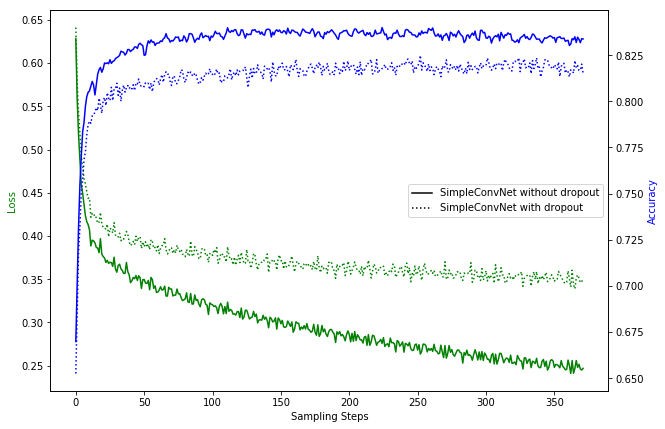
\includegraphics[width=\columnwidth]{overfitting}
  \caption{Plot of the evolution of Loss and Validation Accuracy. Note: The period represented is not the same for both nets, as training with dropout demands more cycles to reach convergence.}
  \vspace{-3mm}
  \label{fig:Validation accuracy vs Loss}
\end{figure}
 
 Dropout forces a neuron to not rely solely on the input it receives from one particular other neuron, but to rely on the input of a random subset of its processors. This leads to the neurons learning more robust features that are still of use when not all of the neurons are present\cite{nielsen_a._1970}. However it seems that for our neural net model the benefit we get by reducing over-fitting by the dropout technique is not worth the loss in accuracy this process causes by generalizing the model. It can be seen on Figure~\ref{fig:Validation accuracy vs Loss} that the version of the net implementing dropout in the fully connected layer (dotted line) fails to reach the same performance on the validation set as the net that does not use dropout. For our final model we are therefore not using dropout.
 

\section{Results and Summary}
Convolutional Neural Networks offer a significant accuracy gain over logarithmic regression. Our implementations deliver consistent accuracy and are not much affected by over-fitting. However, due to their computational complexity special hardware is required for training them. We implemented and tested several preprocessing combinations from the ones mentioned before, some were successful for the models where we trained our own embeddings. However, none of them brought an improvement on accuracy when using the pretrained embeddings. We therefore don't apply any of these preprocessing steps on our data before training for the final submission. Part of this unexpected behaviour of preprocessing could be due to the fact that pretrained GloVe word vectors were trained over a big set of tweets (2.6 billion tweets) and its dictionary contains most of the common words, signs, abbreviations and hashtags in tweets. The results obtained with the model we used with some of the preprocessed methods are summarized in table ~\ref{tab:models_pre_processing}.
To evaluate the models we separated the data (data split) and used it as our validation data set. This estimated accuracy was almost the same as the one obtained in CrowdAI. With this explanation, the best model we obtained is the NGrams net with 1024 channels which we trained over three epochs with batch size 1024 to obtain a score of \textbf{85.1}\% in \textbf{crowdAI} with the ID: 25279 - by Jonas J\"aggi\,,  and \textbf{86.5}\% in our validation test .
Achieving 100\% accuracy is not possible - some tweets don't express a clear emotion, and it is therefore impossible, even for a human, to guess the mood of it.

\begin{table}[H]
  \caption{Text preprocessing - Accuracy on a validation set of 10'000 tweets, using the N-grams network architecture}
   \label{tab:models_pre_processing}
\begin{tabular}{|l|l|}
\hline
\textbf{Preproccessing Method} & \textbf{Accuracy (\%) Test Validation} \\ \hline
Spell Correction & 79.7 \\ \hline
Lemmatization & 82.3\\ \hline
No Preprocessing & 83.4 \\ \hline
\end{tabular}
\end{table}
As we can see from the table above, the preprocessing steps are not improving the accuracy if we use the embeddings of Standford, this is because the embeddings are trained over a huge data-set of over 2.6 billion tweets, which already includes common abbreviations and expressions used on Twitter, and if we actually apply preprocessing steps we loose information that already had a weight defined on the embeddings.

A detailed explanation of how to run the model is in the ``README'' file.

\bibliographystyle{IEEEtran}
\bibliography{literature}

\end{document}
